% Chapter 1

\chapter{Experiments} % Main chapter title

\label{Chapter8}

In this chapter we will display some novel usage in the $ID$ functionalities and qualities.
The following mentioned above qualities will be demonstrated below:

\begin{enumerate}
	\item \textbf{single ID embedding} will be demonstrated by image classification task
	\item \textbf{pairs ID embedding} will be demonstrated by images pairs matching task
\end{enumerate}

For this section we have used an "image retargeting" dataset \cite{ggg}, ehich contains a set of $91$ frame, where each frame has several modifications (each modification applies a different retargeting method)

"http://people.csail.mit.edu/mrub/retargetme/"

\begin{figure}[h] \label{rteregt}
	
	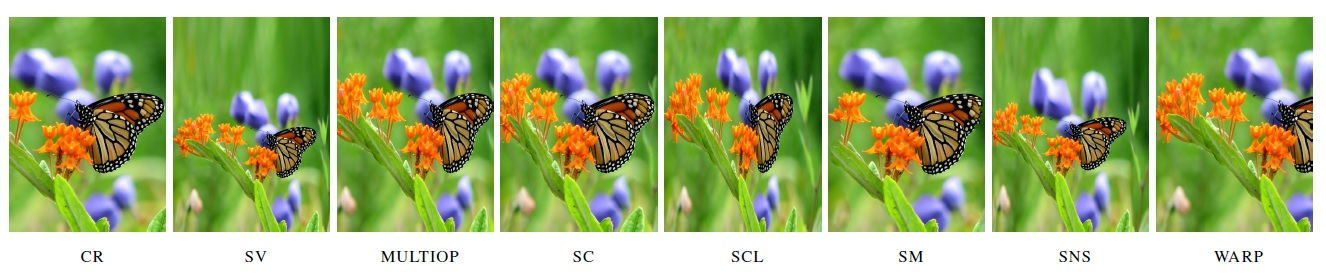
\includegraphics[width=\linewidth,height=12cm,keepaspectratio]{Figures/retargeting}
	\caption[image retargeting example]
	{Example of retargeting the butterfly image to half its size. In this study we evaluate 8 different image	retargeting methods, asking users to compare their results and examine what qualities in retargeted images mattered to them. We also correlate the users’ preferences with automatic image similarity measures. Our findings provide insights on the retargeting problem, and present a clear benchmark for future research in the field.}
	
\end{figure}


\section{experiments procedure}

Each image has 8 various retargeting formations. For each image on dataset we have obtained a single vector descriptor. This descriptor is a SIFT descriptor, calculated on the entire image from its center as shown in figure \ref{single_sift}. 
\\ \\ 
Our set is a $n=128$ length dataset, divided to 91 classes.\\
As described in \ref{Chapter3}, for relatively long vectors such SIFT descriptors, $ID$ method requires memory saving methods. Such method has described in \ref{vbgh} as \textbf{grouping} method. In this method we sample sub-domains from the datasets' vectors, run the $ID$ method separately on each sub-domain, then concatenate the embedded sub-vectors to a flatten embedded vector.\\ 


\begin{figure}[h] \label{single_sift}
	
	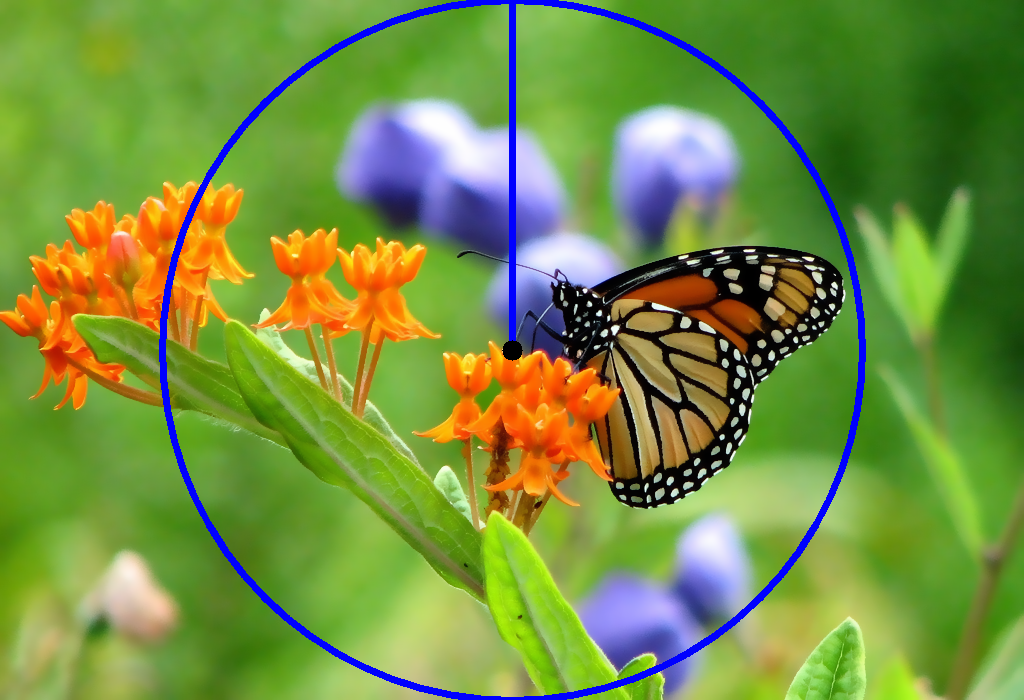
\includegraphics[width=\linewidth,height=12cm,keepaspectratio]{Figures/butterfly_sift}
	\caption[image single sift descriptor]
	{Original butterfly image from retargeting dataset, with an overlay SIFT descriptor on it, as we have measured on every image in the dataset. All SIFT descriptors were taken from the center of the image. Their radius was as the shorter image-side, and their orientation was $+90^{\circ}$.}
	
\end{figure}


We now describe how both cases described above were implemented in this experiment, and observe several behaviors of each task, in relation to some parameters such number of discretization points and number of groups participating in the embedding process.
talk about grouping vectors, \\
about scanning C parameters , \\
about 

\section{classification solution}
\section{pairs matching solution}
